\chapter{Experiments and Results}
\label{chap:experiments}
This chapter presents a series of experiments designed to answer the research questions posed in Chapter~\ref{chap:intro}, focusing on the evaluation of the Mamba-S6 (\acrshort{vms}) model for temporal event spotting in football video. The accuracy and runtime is compared against the \acrshort{tdeed} baseline, investigate the impact of feature dimensionality, and perform a Bayesian hyperparameter sweep to optimize performance.


\section{Experiment 1: Compare accuracy between tdeed and mamba}
\label{sec:experiment1}
The first experiment compares accuracy from \acrshort{tdeed} and \acrshort{vms}. 

\subsection{Setup}
\label{ssec:ex1_setup}
We trained three models on the SoccerNet-V2 dataset \cite{deliege_soccernet-v2_dataset_2021}:  
\begin{itemize}
    \item \acrshort{vms}-80\_20 using an 80\%/20\% train/val split,  
    \item \acrshort{vms}-70\_30 using a 70\%/30\% split, and  
    \item \acrshort{tdeed} with four matches for training and one for validation (equivalent to 80\%/20\%).  
\end{itemize}

All models used default hyperparameters from their original papers. Performance was measured by mean Average Precision (mAP) and mAP@50 under a \(\pm 1\) s tolerance window.

\subsection{Results}
\label{ssec_ex1_results}
\begin{table}[ht]
    \centering
    \begin{tabular}{lcc}
        \toprule
        Model                   & average \acrshort{map} (\%)  & \acrshort{map}@50 (\%) \\
        \midrule
        \acrshort{tdeed}                  &  \textemdash      & 43.00       \\
        \acrshort{vms}-80\_20 (Mamba-S6)   &  \textbf{51.42}   & \textbf{49.38} \\
        \acrshort{vms}-70\_30 (Mamba-S6)   & 48.73            & 46.46       \\
        \bottomrule
    \end{tabular}
    \caption{Accuracy comparison on SoccerNet-V2.}
    \label{tab:results_ex1}
\end{table}
\todo{fill in correct values of tdeed}
\todo{values for vms might be incorrect, run new training to get numbers}

\subsection{Discussion}
\label{ssec:ex1_discussion}

task is made to fit the tdeed model, by fine grained low tolerance for error 

\section{Experiment 2: Compare runtime}
\label{sec:experiment2}

Wall-clock training time for each model on a Tesla A100 \acrshort{gpu} was recorded. Feature extraction was also timed, but separated from the time. \unsure{should I use identical epoch count and batch size?}
\todo{same number of epochs? normalize for number of epochs?} 

\subsection{Setup}
\label{ssec:ex2_setup}

We know mamba is faster than the vit based tdeed

MAMBA training took <3 hours, but data extraction was slow. However also image extraction on tdeed was slow. can say i ignore data preprocessing and just look at 


\section{Experiment 3: Feature increase}
\label{sec:experiment3}
To find out how much the size if the feature vector matters, a model with 1408 features and one with 3200 features is trained on the THUMOS-14 dataset.
InternVideo features have a size of 3200, and is the backbone of the \acrshort{sota} models on paperswithcode.
The \acrshort{vms} models trained on soccernet use 1408 features. 


\subsection{Setup}
\label{ssec:ex3_setup}

To assess the effect of embedding size, two \acrshort{vms} instances were trained on THUMOS-14 \cite{dataset:thumos}: one using 1,408-dimensional VideoMAE features and one using 3,200-dimensional InternVideo embeddings. All other settings, annotations and hyperparameters, remained identical.

The metrics are tracked using \acrlong{wandb} and console logs.
Both models trained for 49 epochs on a Tesla V100-PCIE-32GB \acrshort{gpu}.

\subsection{Results}
\label{ssec:ex3_results}
The 1,408-dimensional model achieved a  \acrshort{map} of \(0.686\), while the 3,200-dimensional model reached a \acrshort{map} of \(0.718\) (a 3.2\% absolute gain). Training times were 1 h 15 min and 1 h 23 min, respectively.

\todo{add wandb plots}

\subsection{Discussion}
\label{ssec:ex3_discussion}
hyperparameters could favor the newer weights


\section{Experiment 4: Hyperparameter optimization}
\label{sec:experiment4}

The fourth experiment is a hyperparameter optimization experiment.
The goal is to find the best hyperparameters for the \acrshort{vms} model on the soccernet dataset.

\subsection{Setup}
\label{ssec:ex4_setup}

\acrlong{wandb} is used to track the hyperparameters and the results for the \acrshort{vms} model trained on SoccerNet-V2 dataset with a 70 \(\%\)-30\(\%\) validation split. A Bayesian optimization algorithm is used to find the best importance and correlation of the hyperparameters. The hyperparameters related to the dataset are the only ones modified. Full details about the hyperparameters can be found in \autoref{label:app_sweep}.

A total of 210 runs across three sweeps of 70 runs each were completed. Because of the fast convergence of \acrshort{vms}--models hyperparameter search was an efficient process. 


\subsection{Results}
\label{ssec:ex4_results}

\begin{figure}
    \centering
    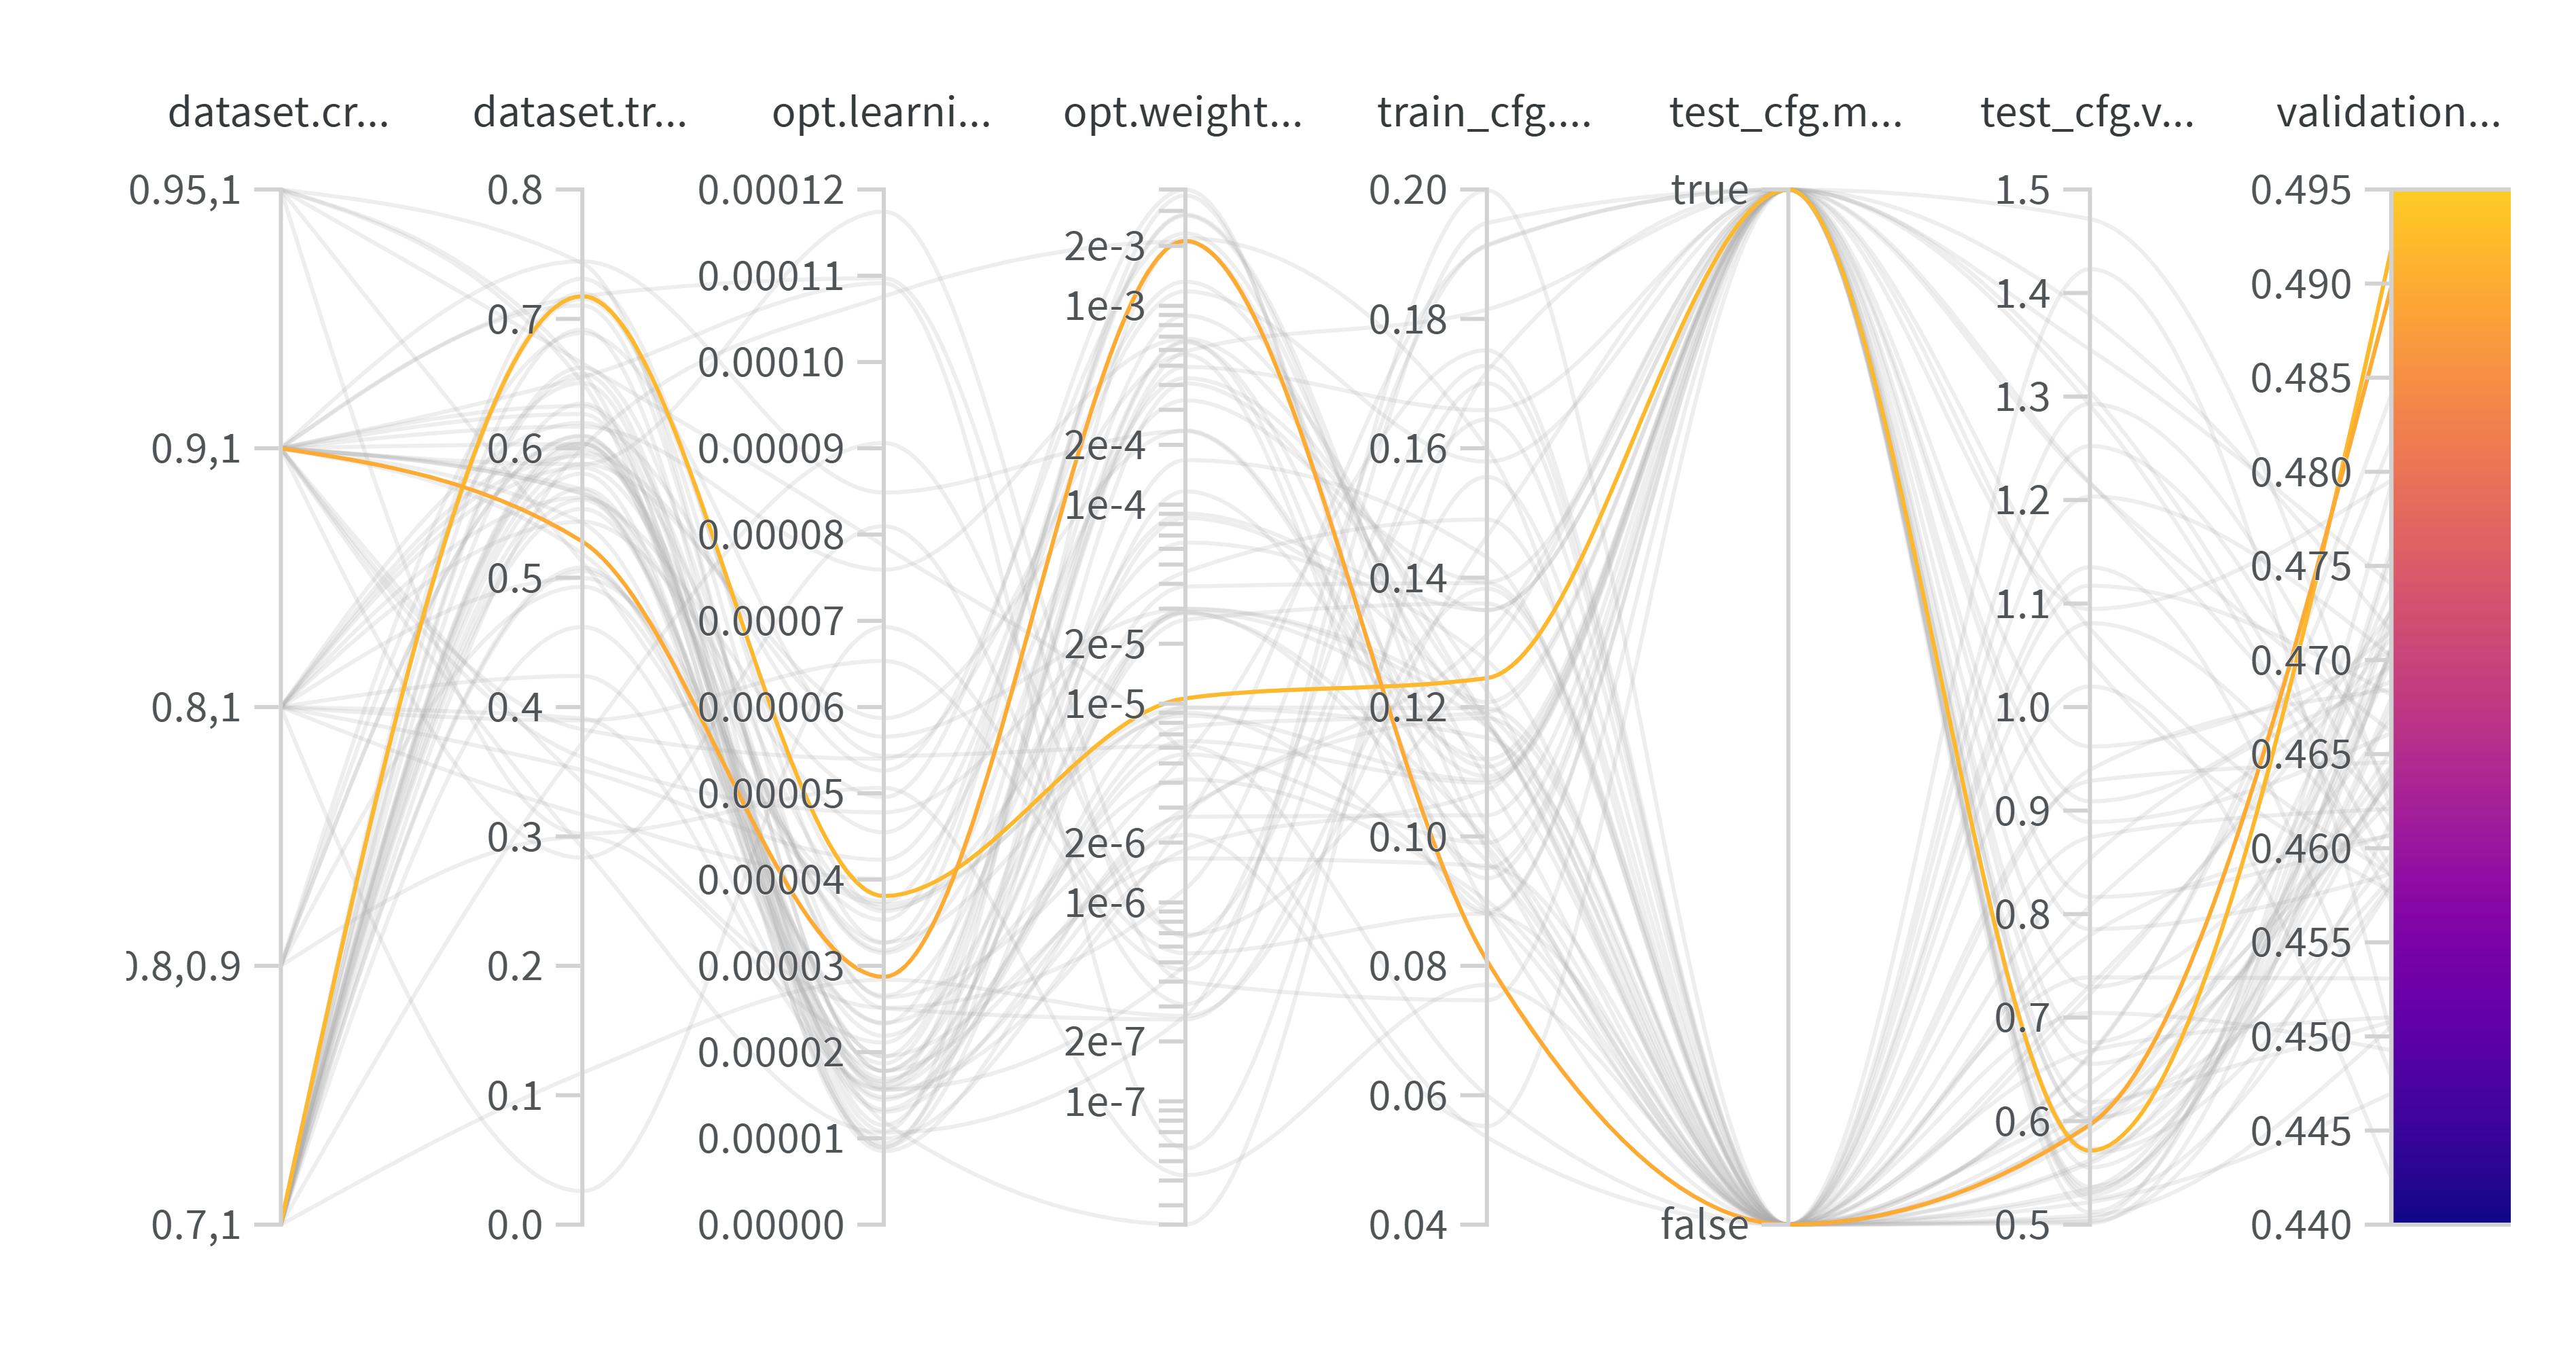
\includegraphics[width=1\linewidth]{figures/sweep_two_best.png}
    \caption{The hyperparameters of the two best results(yellow) compared to all runs(grey) in the thrid sweep. }
    \label{fig:sweep_best_two}
\end{figure}

The sweeps showed a slight improvement to the model. 

Trying to translate the sweep into a single better configration didn't prove useful, but some configurations performed exceptionally better than the rest. But these configurations that worked well, had quite different parameters and was hard to differ. As seen in \autoref{fig:sweep_best_two}, the hyperparameters of the best and second best run in the last sweep differed significantly in their hyperparameters. 

Interpreting the results to create a hyperparameter configuration, as explained in the \autoref{app:sweep_3} the resulting average \acrshort{map} was \(46.77\%\). 

\subsection{Discussion}
\label{ssec:ex4_discussion}
lower learning rate because football is homogeneous
only tune dataset variables
negative/neutral results. why? i think its because features are trained to match the preprocessing timeline. some really good runs
something funny is up with the learning rate



\section{Experiment 5: T-DEED with and without joint training}
\subsection{Setup}
\label{ssec:ex5_setup}

another experiment where I just run array jobs with different train/val splits

\section{Summary}
vms runs on any GPU, but tdeed needs a lot of memory and only runs on premium GPUs.